\chapter{Supplementary material}

\begin{figure}[H]
	\centering
	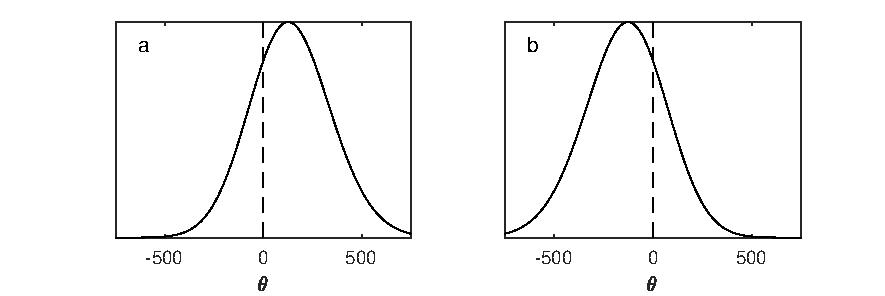
\includegraphics[scale=1.1]{skew_updates.pdf}
	\caption{The skew Gaussian proposal distributions which can be used to positively or negatively bias the parameter update as an alternative to the truncated Gaussian distribution, figure \ref{updates}. The positively skewed distribution (a) is used when the parameter values are deemed too low. The negatively skewed distribution (b) is used when the parameter values are deemed too high. During application the distributions are centered on the current chain and $\omega = 250$.}
	\label{skew-updates}
\end{figure}

\begin{figure}[H]
	\centering
	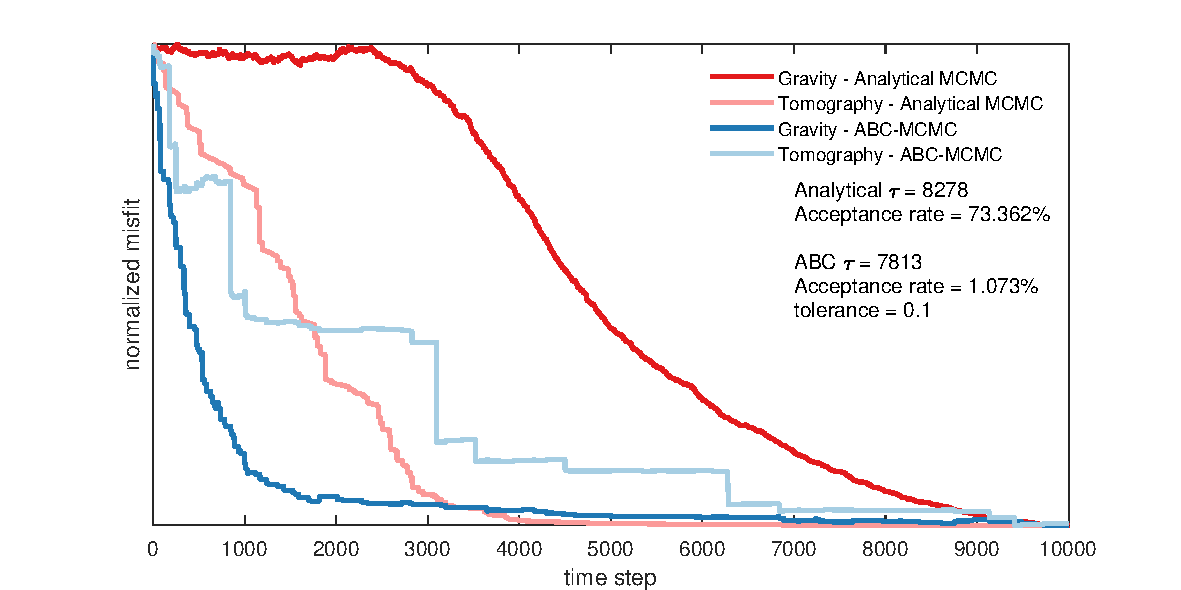
\includegraphics[scale=0.8]{comparison-skew.pdf}
	\caption{Skew Gaussian scheme. The normalized misfit of the chain state during the initial phase (first 10,000 steps) for both datasets, $\Delta g$ and $\Delta t$, and for both methods, an analytically defined posterior sampled by MCMC and ABC-tomography. The `true model' and observed data is plotted in figure \ref{true-model-large-grav} and \ref{true-model-tom}. The increase in the rate of convergence to a low misfit model under ABC-tomography is a result of dynamically selecting, localizing and directly the update at each time step in the Markov chain. The details of the full chain run (100,000 time steps), are also displayed on the figure. $\tau$ is the integrated auto-correlation time. The mean marginal models from ABC-tomography using skew Gaussian updates is plotted in figure \ref{grav-skew} and \ref{tom-skew}.}
	\label{comparison-skew}
\end{figure}

\begin{figure}[H]
	\centering
	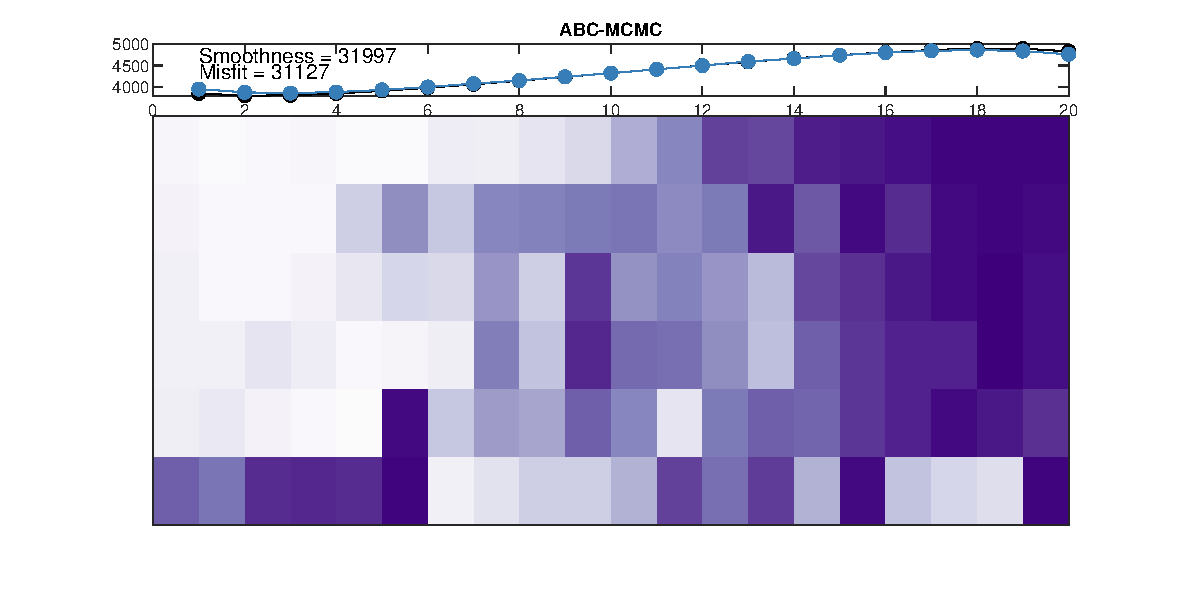
\includegraphics[scale=0.7]{abc_im-skew.pdf}
	\caption{Skew Gaussian scheme. The mean of the marginal ABC posterior, $p_{ABC}(\bm{\theta}|\bm{S}(\bm{y}))$, targeting the `true model' and observed data of figure \ref{true-model-large-grav}. The simulated data generated by this `solution', is plotted, blue, compared to the observed data, black. The misfit during the initial phase for this chain is plotted in figure \ref{comparison-skew}. The corresponding mean marginal $V_p$ model is plotted in figure \ref{tom-skew}.}
	\label{grav-skew}
\end{figure}

\begin{figure}[H]
	\centering
	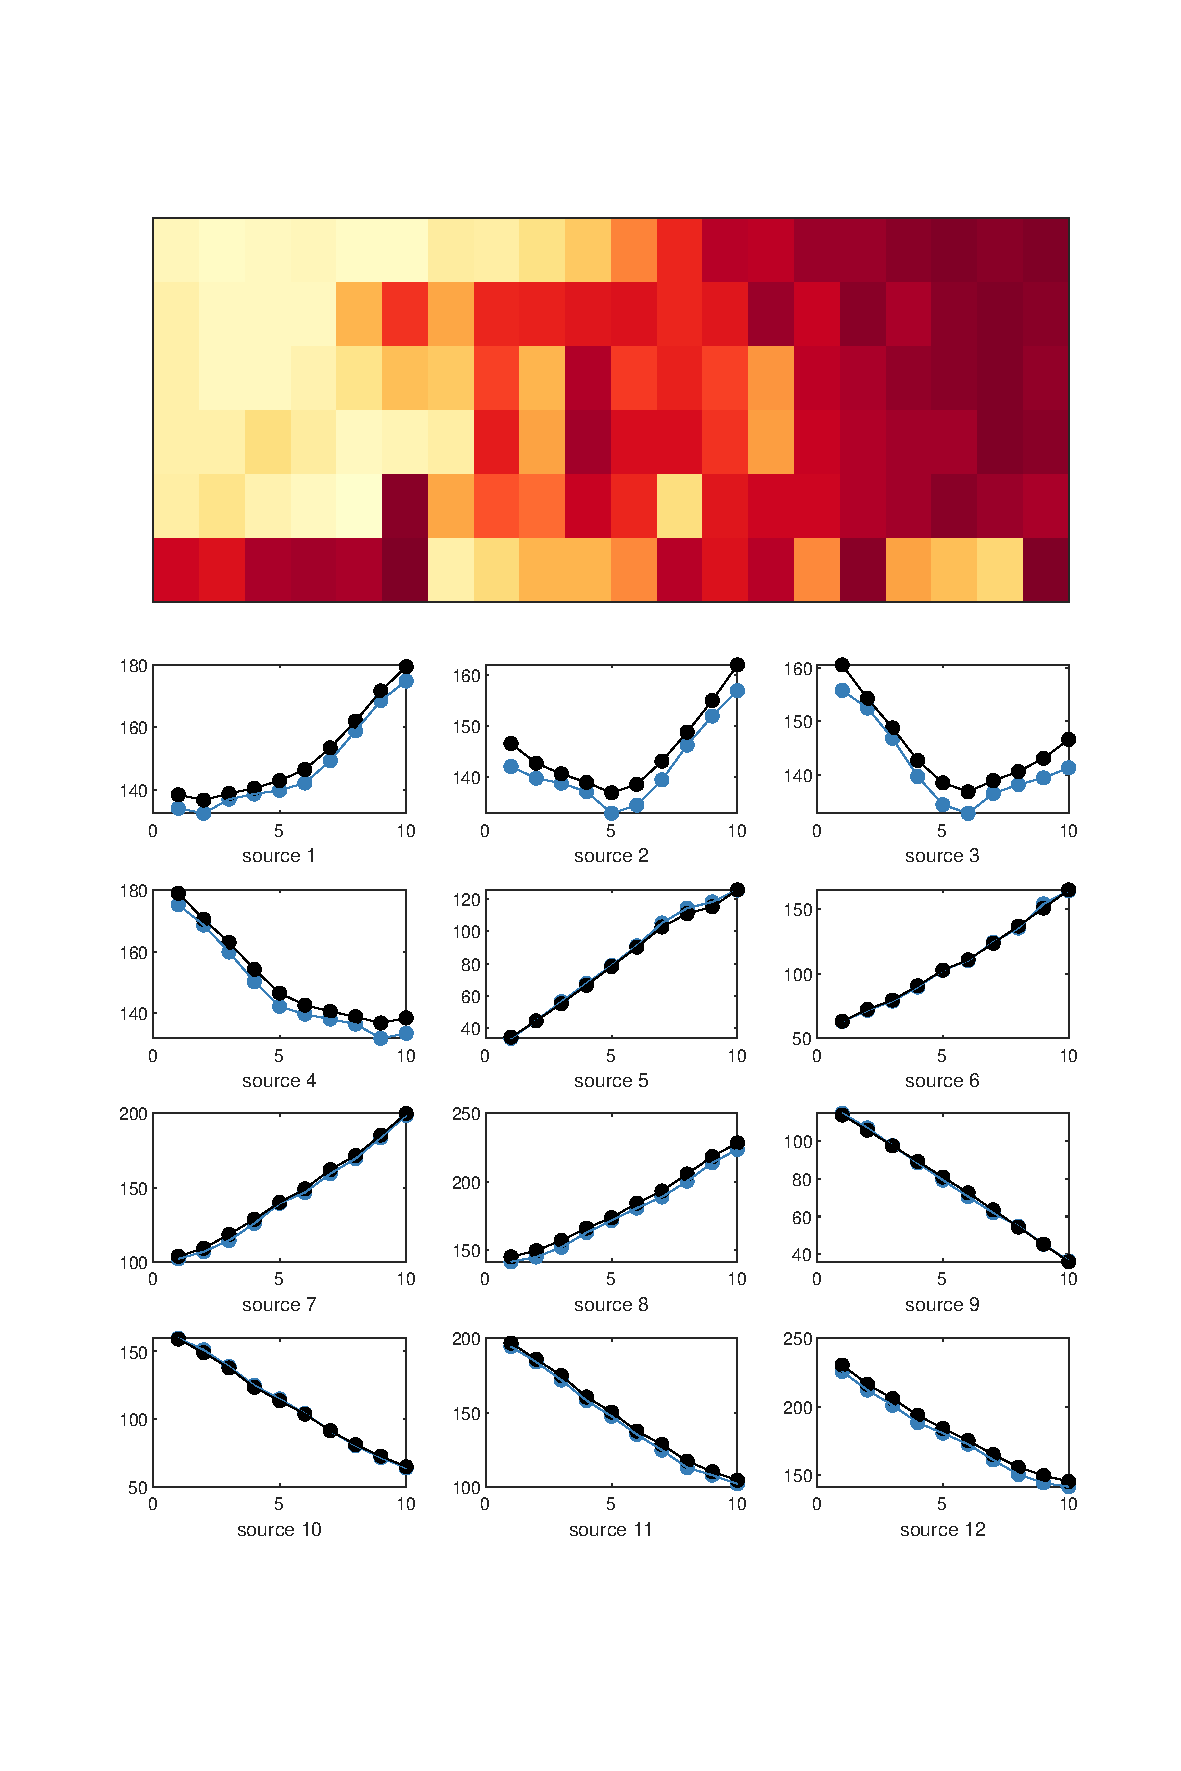
\includegraphics[scale=0.7]{abc-skew.pdf}
	\caption{Skew Gaussian scheme. The mean of the marginal ABC posterior, $p_{ABC}(\bm{\theta}|\bm{S}(\bm{y}))$, targeting the `true model' and observed data of figure \ref{true-model-tom}. The simulated data generated by this `solution', is plotted, blue, compared to the observed data, black. The misfit during the initial phase for this chain is plotted in figure \ref{comparison-skew}. The corresponding mean marginal $\rho$ model is plotted in figure \ref{grav-skew}.}
	\label{tom-skew}
\end{figure}
